\documentclass[nobib]{tufte-handout}

\title{Föreläsning 3: Induktion, lådprincipen, och inklusion-exklusion $\cdot$ 1MA020}

\author[Vilhelm Agdur]{Vilhelm Agdur\thanks{\href{mailto:vilhelm.agdur@math.uu.se}{\nolinkurl{vilhelm.agdur@math.uu.se}}}}

\date{23 januari 2023}


%\geometry{showframe} % display margins for debugging page layout

\usepackage{graphicx} % allow embedded images
  \setkeys{Gin}{width=\linewidth,totalheight=\textheight,keepaspectratio}
  \graphicspath{{graphics/}} % set of paths to search for images
\usepackage{amsmath}  % extended mathematics
\usepackage{booktabs} % book-quality tables
\usepackage{units}    % non-stacked fractions and better unit spacing
\usepackage{multicol} % multiple column layout facilities
\usepackage{lipsum}   % filler text
\usepackage{fancyvrb} % extended verbatim environments
  \fvset{fontsize=\normalsize}% default font size for fancy-verbatim environments

\usepackage{color,soul} % Highlights for text


\include{mathcommands.extratex}

\begin{document}

\maketitle% this prints the handout title, author, and date

\begin{abstract}
\noindent
Vi börjar med att diskutera induktion och induktionsbevis. Sedan nämner vi lådprincipen och ger några tillämpningar av den. Till slut påbörjar vi vår diskussion av inklusion-exklusion.
\end{abstract}

\section{Induktion}

\begin{axiom}[Induktion för heltalen]
  \sidenote[][]{Är detta en sats eller ett axiom? Det beror på vilka axiom du väljer att ta, och hur exakt du definierar vad du menar med ``heltalen''.
  
  Precis vilka axiom vi antar är inte något som vi skall gå in på i denna kursen, det hör snarare hemma i en kurs i logik. Vi nöjer oss att säga, i en sidnot för den intresserade, att enligt Peano är detta ett axiom, men om man resonerar i Zermelo-Fraenkel kan man bevisa att heltalen finns och har denna egenskap.}Antag att $A \subseteq \N$ är någon mängd av heltal. Ifall
  \begin{enumerate}
    \item $1 \in A$, och
    \item för varje $n$, om $n \in A$, så är också $n + 1 \in A$,
  \end{enumerate}
  så är $A = \N$, det vill säga, alla heltal ligger i $A$.
\end{axiom}

Man brukar ofta föredra att tänka på induktion som att det handlar om egenskaper hos eller påståenden om tal -- då säger vi att vi har en egenskap $\phi$, och om vi kan bevisa $\phi(1)$ och kan bevisa att $\phi(n) \rightarrow \phi(n+1)$, så följer det att $\forall n \phi(n)$.

Detta perspektiv är helt ekvivalent med det axiom vi just gav -- om vi låter $A$ vara mängden av tal med egenskapen $\phi$, eller låter $\phi$ vara egenskapen ``talet ligger i $A$''.

\begin{example}
  Bevisa att, för varje $n\geq 1$, $\sum_{i=0}^{n-1} 2^i = 2^n - 1$.

  \begin{proof}
    Låt $A$ vara mängden av alla $n$ sådana att $\sum_{i=0}^{n-1} 2^i = 2^n - 1$.

    Vi ser enkelt att $1 \in A$, eftersom påståendet då blir att $2^0 = 2^1 - 1$, vilket ju är sant.

    Låt oss visa att om $n \in A$ så är också $n+1$ i $A$. Så vi antar likheten för $n$, och vill visa att $\sum_{i=0}^{n} 2^i = 2^{n+1} - 1$. Så om vi skriver vänster led i denna likheten och manipulerar den så ser vi att
    \begin{align*}
      \sum_{i=0}^{n} 2^i &= \sum_{i=0}^{n-1} 2^i + 2^n\\
      &= \left(2^n - 1\right) + 2^n = 2\cdot 2^n - 1 = 2^{n+1} - 1
    \end{align*}
    precis som önskat. Så induktionsprincipen ger oss att likheten håller för alla $n$.
  \end{proof}
\end{example}

\begin{example}
  Bevisa att det finns $n!$ permutationer av längd $n$ från ett alfabete med $n$ bokstäver.
  
  \begin{proof}
    Att det finns exakt en permutation av längd ett från ett alfabete med en bokstav är uppenbart.

    För induktionssteget, antag att vi vet att det finns $n!$ permutationer av längd $n$ från alfabetet $X$, där $\abs{X} = n$. Hur kan vi konstruera en permutation av längd $n+1$ från alfabetet $X\cup\{a\}$? Jo, vi börjar med att välja en permutation av $X$ -- vilket vi per induktionshypotesen kan göra på $n!$ sätt -- och väljer sedan var vi skall stoppa in $a$. Vi har $n+1$ alternativ för plats för $a$, så enligt multiplikationsprincipen har vi $(n+1)n! = (n+1)!$ sätt att skapa en permutation av vårt nya längre alfabete.
  \end{proof}
\end{example}

\begin{remark}[Stark induktion]
  I själva verket kan vi ta som induktionshypotes inte bara att $n \in A$, utan att $[n] \subseteq A$, det vill säga att alla heltal från $1$ till $n$ ligger i $A$. (Eller ``har egenskapen $\phi$'', om vi föredrar den formuleringen.) 
  
  Att göra det antagandet kallas för \emph{stark induktion} -- vilket egentligen är ett missvisande namn, eftersom det är ekvivalent med vanlig induktion, och alltså kan bevisa precis samma saker. Den är alltså inte ett dugg starkare i logisk mening -- men ibland ger den snyggare formuleringar av bevisen.
\end{remark}

\begin{theorem}[Välordningsprincipen]
  För varje mängd $A \subseteq \N$ är antingen $A$ tom, eller så har $A$ ett minsta element.\sidenote[][]{Vi väljer att formulera det här som en sats som följer av induktionsprincipen -- i kursboken är de två separata påståenden, och förra årets anteckningar går i motsatt riktning och bevisar induktion baserat på välordning.S}

  \begin{proof}
    Antag att $A$ är en mängd av heltal utan minsta element -- vi bevisar med (stark) induktion att $A = \emptyset$, genom att bevisa att $A^c = \N$.

    Att $1 \in A^c$ är uppenbart -- ett är det minsta heltalet, så vore ett i $A$ vore det trivialt ett minsta element i $A$.

    Antag nu att $1, 2, \ldots, n \in A^c$. Alltså är inga av heltalen innan $n+1$ med i $A$, så om $n+1$ vore i $A$ skulle det vara $A$s minsta element. Så eftersom $A$ inte har ett minsta element kan inte $n+1$ ligga i $A$.

    Alltså ger oss nu induktionsprincipen att $A^c = \N$, det vill säga $A = \emptyset$, såsom önskat.
  \end{proof}
\end{theorem}

\begin{remark}
  Detta ger upphov till en vanlig bevisteknik.\sidenote[][]{På engelska kallad \emph{proof by infinite descent}.} Antag att vi vill bevisa att alla heltal har en viss egenskap $\phi$. Vi antar då, för motsägelse, att det inte är så -- då måste det finnas ett minsta motexempel, enligt välordningsprincipen. 
  
  Sedan använder vi detta minsta motexempel för att konstruera ett ännu mindre motexempel, och får en motsägelse därur. Att vi kunde skapa ett mindre motexempel motsäger ju nämligen att det vi började med var det minsta exemplet.
\end{remark}

\section{Lådprincipen}

\begin{theorem}[Lådprincipen]\sidenote[][]{Också kallad Dirichlets lådprincip, efter den tyske matematikern Peter Gustav Lejeune Dirichlet. Eller på engelska ``the pigeonhole principle'' -- vilket onekligen är ett mer målande namn än vår svenska lådprincip.}
  Om vi har $m$ stycken objekt som skall fördelas i $n$ lådor, och $m > n$, så kommer någon låda behöva innehålla mer än ett objekt.
\end{theorem}

\begin{example}
  Om det finns tretton studenter i rummet måste åtminstone två av dem fylla år i samma månad. Här är studenterna objekten och årets månader lådorna.\sidenote[][]{Här önskar jag att kursen gick på engelska, så jag kunde skriva, såsom i förra årets anteckningar, att ``students are pigeons''.}
\end{example}

\begin{theorem}[Generaliserade lådprincipen]
  Om vi har $m$ objekt som skall fördelas i $n$ lådor, och $m > kn$, så måste åtminstone en av lådorna innehålla minst $k+1$ objekt.
\end{theorem}

\begin{example}
  Om det finns tjugofem studenter i rummet måste det finnas minst en månad i vilken tre eller fler av dem fyller år.
\end{example}

\begin{example}
  Antag att fem punkter placeras i en liksidig triangel med sidlängd ett. Då finns det två punkter vars avstånd mellan varandra är högst $\frac{1}{2}$.

  Dela upp triangeln i fyra bitar, enligt figuren.
  \begin{figure}
    \centering
    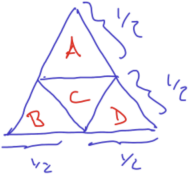
\includegraphics[width = 0.3\textwidth]{graphics/pigeonhole_principle_equilat_triangle.png}
    \caption{Figur tagen från förra årets föreläsningsanteckningar.}
  \end{figure}
  Lådprincipen säger oss att det måste finnas en av dessa bitar som innehåller minst två punkter. Men om de ligger i samma bit måste deras avstånd mellan varandra vara högst $\frac{1}{2}$.
\end{example}

\begin{example}
  För varje mängd av fem punkter på en sfär finns det ett halvklot som innehåller minst fyra av punkterna.

  Välj två av de fem punkterna godtyckligt och rita storcirkeln som passerar genom dem. Denna delar upp jorden i två halvklot, så lådprincipen säger oss att ett av dessa halvklot måste innehålla minst två av de återstående tre punkterna. Det halvklotet har alltså de två punkterna vi ritade storcirkeln genom och minst två punkter till, för totalt minst fyra.
\end{example}

\begin{example}\label{example_R33_is_6}
  I varje grupp av sex personer finns det antingen en grupp av tre personer som alla är vänner eller en grupp av tre personer som alla inte är vänner.\sidenote[][]{Vi antar här att ``är vänner''-relationen är symmetrisk, det vill säga att om jag är vän med dig är du vän med mig. Förhoppningsvis är det antagandet sant på universitetet, även om det inte var sant i mellanstadiet.}

  Välj en godtycklig person i gruppen. Enligt lådprincipen måste det antingen finnas tre personer som hon inte är vän med, eller tre personer som hon är vän med.

  Ifall det finns tre personer som hon inte är vän med har vi två fall -- antingen är alla tre vänner med varandra, i vilket fall vi är klara, eller så finns det ett par av dem som inte känner varandra. Men i så fall bildar det paret, tillsammans med vår första person, en grupp av tre personer som alla inte känner varandra.

  Ifall det finns tre personer som hon är vän med resonerar vi på samma vis. Antingen är ingen av de tre personerna vänner med varandra, i vilket fall vi hittat vår grupp, eller så finns det ett par som känner varandra, och i så fall bildar det paret tillsammans med vår första person en triangel som känner varandra.
\end{example}

Vad vi just studerat är det enklaste fallet av Ramseys sats.\sidenote[][]{Namngiven efter Frank P. Ramsey, som var en fascinerande person som hann bli vän med Wittgenstein och Keynes och finna viktiga resultat inom ekonomi, matematik, och filosofi innan sin bortgång vid 26 års ålder.} Låt oss definiera en lite mer allmän version av problemet.

\begin{definition}
  För varje par av positiva heltal $r$ och $s$ är $R(r,s)$ det minsta antalet personer man behöver bjuda in på en fest för att det skall finnas antingen en grupp av $r$ personer som alla känner varandra, eller en grupp av $s$ personer där ingen känner någon annan i gruppen.\sidenote[][]{Eller mer formellt, formulerat i termer av grafer: (Vi har inte introducerat sådana än, men nästan hälften av er har ju läst kursen i grafteori.)
  
  $R(r,s)$ är det minsta talet sådant att varje graf $G$ med minst $R(r,s)$ noder antingen innehåller en inducerad kopia av $K_r$ eller har en inducerad kopia av $K_s$ i $G^c$, komplementgrafen till $G$.}
\end{definition}

Vad Exempel \ref{example_R33_is_6} visade är alltså att $R(3,3) = 6$. Vad Ramseys sats säger i allmänhet är att $R(r,s)$ är ändligt.\sidenote[][]{Problemet att beräkna exakt vad $R(r,s)$ är är extremt svårt -- vi vet att $R(4,4) = 18$, men kan inte bestämma $R(5,5)$ mer exakt än att det är mellan $43$ och $48$.}

\begin{theorem}[Ramseys sats]\label{ramseys_theorem}
  För varje $r, s \geq 1$ är $R(r,s) < \infty$.
\end{theorem}

\begin{theorem}[Erd\H{o}s-Szekeres]
  För alla $r,s \geq 1$ gäller det att varje följd av $(r-1)(s-1) + 1$ distinkta reella tal antingen innehåller en ökande delföljd av längd $r$ eller en minskande delföljd av längd $s$.

  \begin{proof}
    Kalla vår talföljd $n_1, n_2, \ldots, n_{(r-1)(s-1)+1}$. Ge varje $n_i$ en etikett $(a_i, b_i)$ som följer: $a_i$ är längden av den längsta ökande delföljden som slutar i $n_i$, och $b_i$ är längden av den längsta minskande delföljden som slutar i $n_i$.\sidenote[][]{Här menar vi med ``slutar i'' inte att de inte kan fortsättas längre med något $n_j$ för $j > i$, bara att vi mäter längden av följderna fram till $i$.}

    Vi hävdar att alla tal $n_i$ får distinkta etiketter. Överväg paret $n_i, n_j$ för $i < j$ -- om $n_i < n_j$ kan vi fortsätta den längsta ökande delföljden som slutar i $n_i$ genom att lägga till $n_j$, så $a_j \geq a_i + 1$. Likaledes, om $n_i > n_j$ kan vi fortsätta den längsta minskande delföljden som slutar i $n_i$ genom att lägga till $n_j$, så $b_j \geq b_i + 1$.

    Antag nu för motsägelse att det inte finns någon ökande delföljd av längd $r$, och ingen minskande delföljd av längd $s$. Då måste $1 \leq a_i \leq r-1$ och $1\leq b_i \leq s-1$ för alla $i$.\sidenote[][]{$a_i, b_i \geq 1$ eftersom $n_i$ självt är en delföljd som är både minskande och ökande.}

    Alltså finns det $(r-1)(s-1)$ tillgängliga etiketter att tilldela till $(r-1)(s-1) + 1$ stycken objekt, och alla objekten måste få distinkta etiktter. Lådprincipen säger oss att detta är omöjligt, och vi har vår motsägelse.
  \end{proof}
\end{theorem}

\section{Inklusion-exklusion}

I matematiska institutionens fikarum för de anställda brukar det finnas äpplen, klementiner, och bananer i fruktlådorna. Om någon säger dig att det för tillfället finns femton runda frukter och tio frukter som inte går att odla i Sverige i lådorna, kan du räkna ut hur många frukter det finns?

Det kan du förstås inte -- problemet är att en klementin tillhör båda kategorierna, så om det finns tio klementiner finns det totalt femton frukter (tio klementiner och fem äpplen), men om det finns noll klementiner finns det totalt tjugofem frukter (femton äpplen och tio bananer). Utan informationen om hur många klementiner det finns kan svaret på frågan variera.

Om vi låter $A$ vara mängden av runda frukter och $B$ vara mängden av frukter som inte kan odlas i Sverige är vad vi har observerat att\sidenote[][]{Jämför detta med additionsprincipen, som i en formulering säger att $\abs{A \coprod B} = \abs{A} + \abs{B}$. När vi introducerade den var vi noggranna med skillnaden mellan $\coprod$ och $\cup$, och sade att vi skulle återkomma till vad som händer om $A$ och $B$ kan dela element.

Detta är vår återkomst.}
$$\abs{A \cup B} = \abs{A} + \abs{B} - \abs{A \cap B}.$$

En dag kommer en administratör på idén att citroner faktiskt också är en frukt, och berättar för dig att idag finns det tio runda frukter, elva som inte kan odlas i Sverige, och sju \emph{gula frukter}. Du blir förvirrad och går hem och ritar ett Venndiagram över frukter.\sidenote[][]{Nästa morgon får du reda på att det nu dessutom finns gula äpplen, päron, stjärnfrukt, och Xoconostler. Du skriver en arg insändare i UNT om vad universitetet egentligen lägger sin budget på.}

Formeln du kommer på efter att ha studerat ditt Venndiagram är att
\begin{align*}
  \abs{A \cup B \cup C} &= \abs{A} + \abs{B} + \abs{C}\\
  &\qquad - \abs{A \cap B} - \abs{A \cap C} - \abs{B \cap C}\\
  &\qquad + \abs{A \cap B \cap C}.
\end{align*}

Innan den fruktgalna administratören hinner lägga till ännu en absurd kategori av frukt undsätter dig din kombinatoriklärare med följande sats:
\begin{theorem}[Inklusion-exklusion]\label{theorem_inclusion_exclusion}
  För varje samling av mängder $A_1, \ldots, A_n$ gäller det att
  $$\abs{\bigcup_{i=1}^n A_i} = \sum_{k=1}^{n} (-1)^{k-1}\left(\sum_{\substack{I \subseteq [n]\\\abs{I} = k}} \abs{\bigcap_{i \in I} A_i}\right),$$
  eller, uttryckt mindre kompakt, att
  \begin{align*}
    \abs{\bigcup_{i=1}^n A_i} = \sum_{i=1}^n &\abs{A_i}\\
    & - \sum_{\{i,j\} \in [n]} \abs{A_i \cap A_j}\\
    & + \sum_{ \{i, j, k\} \in [n] } \abs{A_i \cap A_j \cap A_k}\\
    & - \ldots\\
    & + (-1)^{n-1}\abs{A_1\cap A_2\cap\ldots\cap A_n}.
  \end{align*}
\end{theorem}

Innan vi bevisar detta behöver vi definiera ett väldigt nyttigt verktyg som vi kommer använda i beviset.

\begin{definition}
  Antag att $A \subseteq X$ är två mängder. Vi definierar \emph{indikatorfunktionen} $\indSet{A}: X \to \{0,1\}$ \emph{för mängden $A$} som
  $$\indSet{A}(x) = \begin{cases}
    1  & x \in A \\
    0 & x \not\in A.
  \end{cases}$$

  Den är alltså ett om och endast om dess argument ligger i $A$. Vi kan observera några grundläggande egenskaper hos dessa funktioner:
  \begin{itemize}
    \item $\indSet{A}(x)\indSet{B}(x) = \indSet{A\cap B}(x)$
    \item $1 - \indSet{A}(x) = \indSet{X \setminus A}(x)$
    \item $\abs{A} = \sum_{x \in A} \indSet{A}(x)$
    \item $(\indSet{A}(x))^n = \indSet{A}(x)$ för alla $n \neq 0$.
  \end{itemize}
\end{definition}

Med denna definition gjord kan vi nu resonera algebraiskt om mängder och deras kardinalitet, och kan alltså ge ett algebraiskt bevis av inklusion-exklusion-principen.

\begin{proof}[Algebraiskt bevis av Teorem \ref{theorem_inclusion_exclusion}]
  Låt $X = \cup_{i=1}^n A_i$. Vi ser att
  $$\abs{\bigcup_{i=1}^n A_i} = \sum_{x \in X} \indSet{X}(x)$$
  så vi kan fokusera på varje punkt i taget, och visa att den räknas rätt antal gånger.

  Studera nu uttrycket
  $$(\indSet{X}(x) - \indSet{A_1}(x))(\indSet{X}(x) - \indSet{A_2}(x))\ldots(\indSet{X}(x) - \indSet{A_n}(x))$$
  och observera att det måste vara identiskt noll. För varje element $x\in X$ ligger ju i något $A_i$, så produkten innehåller en term $\indSet{X}(x) - \indSet{A_i}(x) = 1 - 1 = 0$.

  Vad får vi om vi multiplicerar ut detta uttrycket? Jo, vi får en term per mängd $I \subseteq [n]$, där vi valt sidan $\indSet{X}(x)$ för $i\not\in I$ och valt sidan $-\indSet{A_i}(x)$ för $i \in I$.\sidenote[][]{Jämför med hur vi resonerade om att multiplicera ut en produkt när vi bevisade binomialsatsen.} Vi vet att uttrycket är noll, så vad vi får är likheten
  $$\sum_{I \subseteq [n]} \left(\indSet{X}(x)\right)^{n - \abs{I}}\prod_{i\in I}\left(-\indSet{A_i}(x)\right) = 0$$
  och om vi skriver termerna för $I = \emptyset$ och $I = [n]$ separat har vi likheten
  $$\prod_{i=1}^{n} (-\indSet{A_i}(x)) + \left(\sum_{\substack{I \subset [n]\\\emptyset \neq I \neq [n]}} \left(\indSet{X}(x)\right)^{n - \abs{I}}\prod_{i\in I}\left(-\indSet{A_i}(x)\right)\right) + \left(\indSet{X}(x)\right)^n = 0$$

  Vi vet av våra räkneregler för indikatorfunktioner att $\indSet{X}(x)^{n-\abs{I}} = \indSet{X}(x)$, eftersom vi plockat ut termen där exponentn blir noll. Den återstående $\indSet{X}(x)$ kan vi bli av med via en annan räkneregel -- vi vet att $\indSet{X}(x)\indSet{A_i}(x) = \indSet{X \cap A_i}(x) = \indSet{A_i}(x)$, eftersom $A_i \subseteq X$, och vi kan göra detta eftersom vi plockat ut termen där vi inte har någon $A_i$ att absorbera in den i. 
  
  Om vi tillämpar dessa förenklingar, flyttar ut minustecknet ur produkten och ser att $\indSet{X}(x)^n = \indSet{X}$, blir vad som återstår
  $$(-1)^n\prod_{i=1}^{n} \indSet{A_i}(x) + \sum_{\substack{I \subset [n]\\\emptyset \neq I \neq [n]}} (-1)^{\abs{I}}\prod_{i\in I}\left(\indSet{A_i}(x)\right) + \indSet{X}(x) = 0.$$
  
  Nu kan vi flytta ihop första och andra termen under en summa, eftersom bägge inte innehåller någon $\indSet{X}(x)$. Om vi gör det, och flyttar över den summan på andra sidan, så får vi att
  $$\indSet{X}(x) = \sum_{\substack{I \subseteq [n]\\I \neq \emptyset}} (-1)^{\abs{I} + 1}\left(\prod_{i\in I} \indSet{A_i}(x)\right).$$

  Om vi använder räkneregeln att $\indSet{A}(x)\indSet{B}(x) = \indSet{A\cap B}(x)$ på produkten här och sedan summerar likheten över alla $x\in X$ så får vi att
  $$\sum_{x\in X} \indSet{X}(x) = \sum_{\substack{I \subseteq [n]\\I \neq \emptyset}} (-1)^{\abs{I} + 1}\left(\sum_{x\in X} \indSet{\bigcap_{i\in I} A_i}(x)\right)$$
  vilket, om vi använder oss av att $\sum_{x\in X} \indSet{A}(x) = \abs{A}$, blir
  $$\abs{X} = \sum_{\substack{I \subseteq [n]\\I \neq \emptyset}} (-1)^{\abs{I} + 1}\abs{\bigcap_{i\in I} A_i}$$
  vilket vi någorlunda enkelt ser är ett annat sätt att skriva formeln vi var ute efter.
\end{proof}

\begin{example}
  Hur många heltalslösningar finns det till $x_1 + x_2 + x_3 = 20$, där $0 \leq x_1 \leq 8$, $0 \leq x_2 \leq 10$, och $0 \leq x_3 \leq 12$?

  Låt
  $$X = \left\{(x_1, x_2, x_2) \in \Z_{\geq 0}^3 \given x_1 + x_2 + x_2 = 20\right\}$$
  och låt
  $$A_1 = \left\{(x_1, x_2, x_2) \in \Z_{\geq 0}^3 \given x_1 + x_2 + x_2 = 20, x_1 > 8\right\},$$
  $$A_2 = \left\{(x_1, x_2, x_2) \in \Z_{\geq 0}^3 \given x_1 + x_2 + x_2 = 20, x_2 > 10\right\},$$
  $$A_3 = \left\{(x_1, x_2, x_2) \in \Z_{\geq 0}^3 \given x_1 + x_2 + x_2 = 20, x_3 > 12\right\}$$
  vara mängder av \emph{dåliga} lösningar, som inte uppfyller våra krav.

  Vad vi vill göra är alltså att räkna ut $\abs{\left(A_1 \cup A_2 \cup A_3\right)^c} = \abs{X} - \abs{A_1 \cup A_2 \cup A_3}$. 
  Inklusion-exklusion säger oss att
  \begin{align*}
    \abs{A_1 \cup A_2 \cup A_3} = \abs{A_1}& + \abs{A_2} + \abs{A_3}\\
    &- \abs{A_1 \cap A_2} - \abs{A_1 \cap A_3} - \abs{A_2 \cap A_3}\\
    &+ \abs{A_1 \cap A_2 \cap A_3}
  \end{align*}
  så vad vi behöver göra är att räkna ut $\abs{X}$ och storleken på dessa snitten.

  Vi såg redan i förra föreläsningen, i biten om omordningar, hur man räknar ut $\abs{X}$ -- det ges av $\binom{20+3-1}{3-1}$. För att räkna ut $A_1$ tänker vi att vi börjar med att ge nio mynt till $x_1$, och fördelar de återstående elva mynten godtyckligt. Vår formel ger oss att detta kan göras på $\binom{11+3-1}{3-1}$ sätt. Så, om vi tillämpar detta på alla tre mängderna ser vi att
  $$\abs{A_1} = \binom{11+3-1}{3-1}, \quad\abs{A_2} = \binom{9+3-1}{3-1}, \quad\abs{A_3} = \binom{7+3-1}{3-1}.$$

  De större snitten är enklare att räkna ut -- för $A_1\cap A_2$ måste vi dela ut nio mynt till $x_1$, och sedan elva mynt till $x_2$, så vi har inga mynt kvar att dela ut fritt, och $\abs{A_1 \cap A_2} = 1$. För de två andra snitten ser vi att $9 + 13 > 20$ och $11 + 13 > 20$, så de snitten måste vara tomma. Likaledes måste snittet av alla tre mängderna vara tomt.\sidenote[][]{Detta följer så klart också redan av observationen att $A_1 \cap A_3 = \emptyset$ -- att snitta med en till mängd kan ju inte lägga till fler element.}

  Sätter vi tillbaka dessa talen i inklusion-exklusion-formeln ser vi att vi fått att
  \begin{align*}
    \abs{\left(A_1 \cup A_2 \cup A_3\right)^c} &= \abs{X} - \abs{A_1 \cup A_2 \cup A_3}\\
    &= \binom{20 + 3 - 1}{3 - 1} - \Bigg(\binom{11+3-1}{3-1}+ \binom{9+3-1}{3-1}\\
    &\qquad\qquad + \binom{7+3-1}{3-1}- 1\Bigg)\\
    &= 63.
  \end{align*}
\end{example}

\subsection{Derangemang}

\begin{definition}
  Ett \emph{derangemang}\sidenote[][]{På engelska \emph{derangement}.} av längd $n$ är en permutation $\sigma$ av längd $n$ ur alfabetet $[n]$, sådan att $\sigma(k) \neq k$ för alla $k$.
\end{definition}

\begin{theorem}
  Det finns
  $$n!\sum_{i=0}^{n} \frac{(-1)^i}{i!}$$
  derangemang av längd $n$.\sidenote[][]{Ni kanske känner igen summan här som en partialsumma av Taylorexpansionen av $e^x$ då $x = -1$ -- så antalet derangemang är mycket nära $\frac{n!}{e}$ för stora $n$.}

  \begin{proof}
    Låt $S_n$ vara mängden av alla permutationer av $[n]$ av längd $n$, och för varje $i$,
    $$A_i = \left\{\sigma \in S_n \given \sigma(i) = i\right\}$$
    så att vi vill räkna antalet element i $S_n \setminus \bigcup_{i=1}^n A_i$.

    Att $\abs{S_n} = n!$ lärde vi oss redan första föreläsningen, och inklusion-exklusion ger oss att
    $$\abs{\bigcup_{i=1}^n A_i} = \sum_{k=1}^{n} (-1)^{k-1}\left(\sum_{\substack{I \subseteq [n]\\\abs{I} = k}} \abs{\bigcap_{i \in I} A_i}\right).$$

    Så vad vi behöver göra är att lista ut vad $\abs{\bigcap_{i \in I} A_i}$ är för varje givet $I \subseteq [n]$. Detta snittet blir precis mängden av permutationer sådana att $\sigma(i) = i$ för varje $i\in I$. Så för att skapa en sådan måste vi först sätta $\sigma(i) = i$ för dem, och sedan kan vi välja en ordning fritt för de återstående $n-k$ platserna. Detta kan vi alltså göra på $(n-k)!$ sätt.

    För varje $k$ finns det $\binom{n}{k}$ stycken mängder $I$, så sammantaget måste vi ha att 
    \begin{align*}
      \sum_{k=1}^{n} (-1)^{k-1}\left(\sum_{\substack{I \subseteq [n]\\\abs{I} = k}} \abs{\bigcap_{i \in I} A_i}\right) &= \sum_{k=1}^{n} (-1)^{k-1}\binom{n}{k} (n-k)!\\
      &= \sum_{k=1}^{n} (-1)^{k-1}\frac{n!}{k!(n-k)!}(n-k)!\\
      &= \sum_{k=1}^{n} (-1)^{k-1}\frac{n!}{k!}
    \end{align*}
    så att
    \begin{align*}
      \abs{S_n \setminus \bigcup_{i=1}^n A_i} &= \abs{S_n} - \abs{\bigcup_{i=1}^n A_i}\\
      &= n! - \sum_{k=1}^{n} (-1)^{k-1}\frac{n!}{k!} = n!\sum_{i=0}^{n} \frac{(-1)^i}{i!}
    \end{align*}
    såsom vi önskade visa.
  \end{proof}
\end{theorem}

\section{Övningar}

\begin{xca}
  Ge ett induktionsbevis av Teorem \ref{theorem_inclusion_exclusion}, teoremet där vi bevisar inklusion-exklusion-principen.
\end{xca}

\begin{xca}
  Antag att du äger svarta, gråa, blåa, och vita strumpor. Tyvärr är du väldigt oorganiserad, så du förvarar dem inte i par. Varje morgon sträcker du dig ner i din strumplåda och tar upp strumpor slumpmässigt, en i taget, tills du har ett matchande par av någon färg.

  Hur många strumpor kan du som mest behöva plocka upp?
\end{xca}

\begin{xca}
  Man kan visa, med samma metod som vi använde i Exempel \ref{example_R33_is_6}, att
  $$R(r,s) \leq R(r-1,s) + R(r, s-1)$$
  för alla $r, s \geq 2$.

  Använd denna olikhet för att bevisa Ramseys sats, Teorem \ref{ramseys_theorem}.\sidenote[][]{Ledtråd: Induktion. Vad kan basfallet tänkas vara?}
\end{xca}

\begin{xca}
  Beteckna antalet derangemang av $n$ med $d_n$. Ge ett kombinatoriskt bevis\sidenote[][]{Ledtråd: För ett givet derangemang $\sigma$ av längd $n$, låt $k$ vara det tal som skickas till $1$. Det finns två fall: Antingen är $\sigma(1) = k$ eller inte. Hur många derangemang finns det i varje fall?} för att
  $$d_n = (n-1)(d_{n-1} + d_{n-2}).$$
\end{xca}

\begin{xca}
  Hur många heltalslösningar har ekvationen $x_1 + x_2 + x_3 + x_4 = 29$ om vi kräver $0 \leq x_i \leq 9$ för alla $i$?
\end{xca}

\begin{xca}
  Antag att den fruktgalna administratören i vårt exempel till slut introducerat tio olika kategorier av frukt. Hur många termer kommer formeln för inklusion-exklusion ha när $n = 10$?
\end{xca}

%\bibliography{references}
%\bibliographystyle{plainnat}

\end{document}
